\documentclass[12pt]{article}

\title{ECE4063 - Image Thresholding}
%\subtitle{Progress Report}
\author{Emmanuel Jacyna - 24227498 \and James Anastasiou - 23438940}
\date{\today}

\usepackage[T1]{fontenc}
\usepackage[utf8]{inputenc}
\usepackage{rotating}
\usepackage{subfig}

\usepackage{graphicx}
\usepackage{tabularx}
\usepackage{float}
\usepackage{amsmath}
\usepackage{listings}
\bibliographystyle{unsrt}


\begin{document}
\pagestyle{myheadings}
  \maketitle
  \tableofcontents
  \section{Introduction}
  This document represents our findings for Assignment 2 of ECE4063. It is organised into three major sections, assumptions, solution documentation, and a discussion of potential improvements to the project.\\
  
  The task at hand is to perform binary thresholding on an image for use in a bionic eye. The target platform is an Altera Cyclone II FPGA. In order to threshold the image, a histogram of the pixel greyscale values is calculated and used to find the 50th percentile grey scale value. This value is then used to decide whether to colour pixels white or black, performing a total threshold.
  
  \section{Assumptions}
  When thresholding images, we assume that an image where 99.9\% of pixels are one value is meaningless to threshold. In the case of the Altera DE2 board with Terasic camera module, the small variation in value is likely to be because of pixel noise. We also believe that as the target is a human vision system, 100\% accuracy is not necessarily the goal, as we prefer an image that makes sense to the human eye. This design decision allowed for a simplification of the logic circuit required to determine the most accurate thresholding value. 
  
  We also assumed that Model Sim testbenches are 100\% completely accurate representations of reality. This assumption was routinely called into question, however after fixing a number of other assumptions, this sole assumption was found to be a valid assumption.
  
  \section{Documentation}
  \subsection{RGB to Grayscale conversion}


  
  \subsection{Histogram Module}
  The histogram module was 
  
  
  \subsection{Cumulative Histogram Module}
  
  \subsection{Thresholding Module}
  \subsubsection{Description}
  The thresholding module is very simple. All it needs to do is take in an 8 bit greyscale value and output either a white (255) if the value is above the threshold, or a black (0) if the value is below the threshold. This is accomplished by hooking up a comparator to a multiplexer.
  
  \subsubsection{RTL Diagram}
  \begin{figure}[H]
    \centering{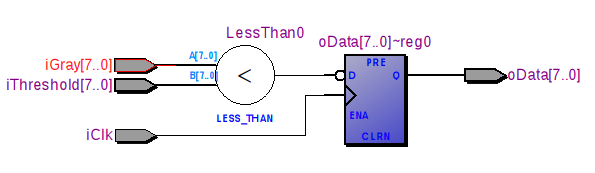
\includegraphics[scale=.8]{Images/ThresholderRTL.png}}
    \caption{Thresholding module RTL}
    \label{fig:thresholder_rtl}
  \end{figure}
  
  
  \subsection{Displaying things}
  \subsubsection{Description}
  In order to display the greyscale image, histogram, cumulative histogram, and thresholded image, we wrote a module to handle multiplexing between them using the switches on the DE2 board, called Arbitrator. This module takes in pixel outputs from the various modules and multiplexes them depending on the switch positions. In order to display images, we simply piggyback on the \(X\_Cont\) and \(Y\_Cont\) signals and modify the \(wr1\_data\) and \(wr2\_data\) inputs to the SDRAM with the appropriate pixel data. \\
      
  Displaying the actual histogram data requires slightly more effort. First we need to extract the histogram data from the histogram RAM and convert the histogram bin contents into pixels for display on the screen. To do this we have a module called HistogramDisplayer. This module takes in the \(Y\_Cont\) signal and uses it to index the histogram RAM. Based on the value obtained from the RAM, it scales the histogram value, and uses the \(X\_Cont\) signal to determine the length of the line to be displayed. 
  \subsubsection{RTL Diagram}
    \begin{figure}[H]
    \centering{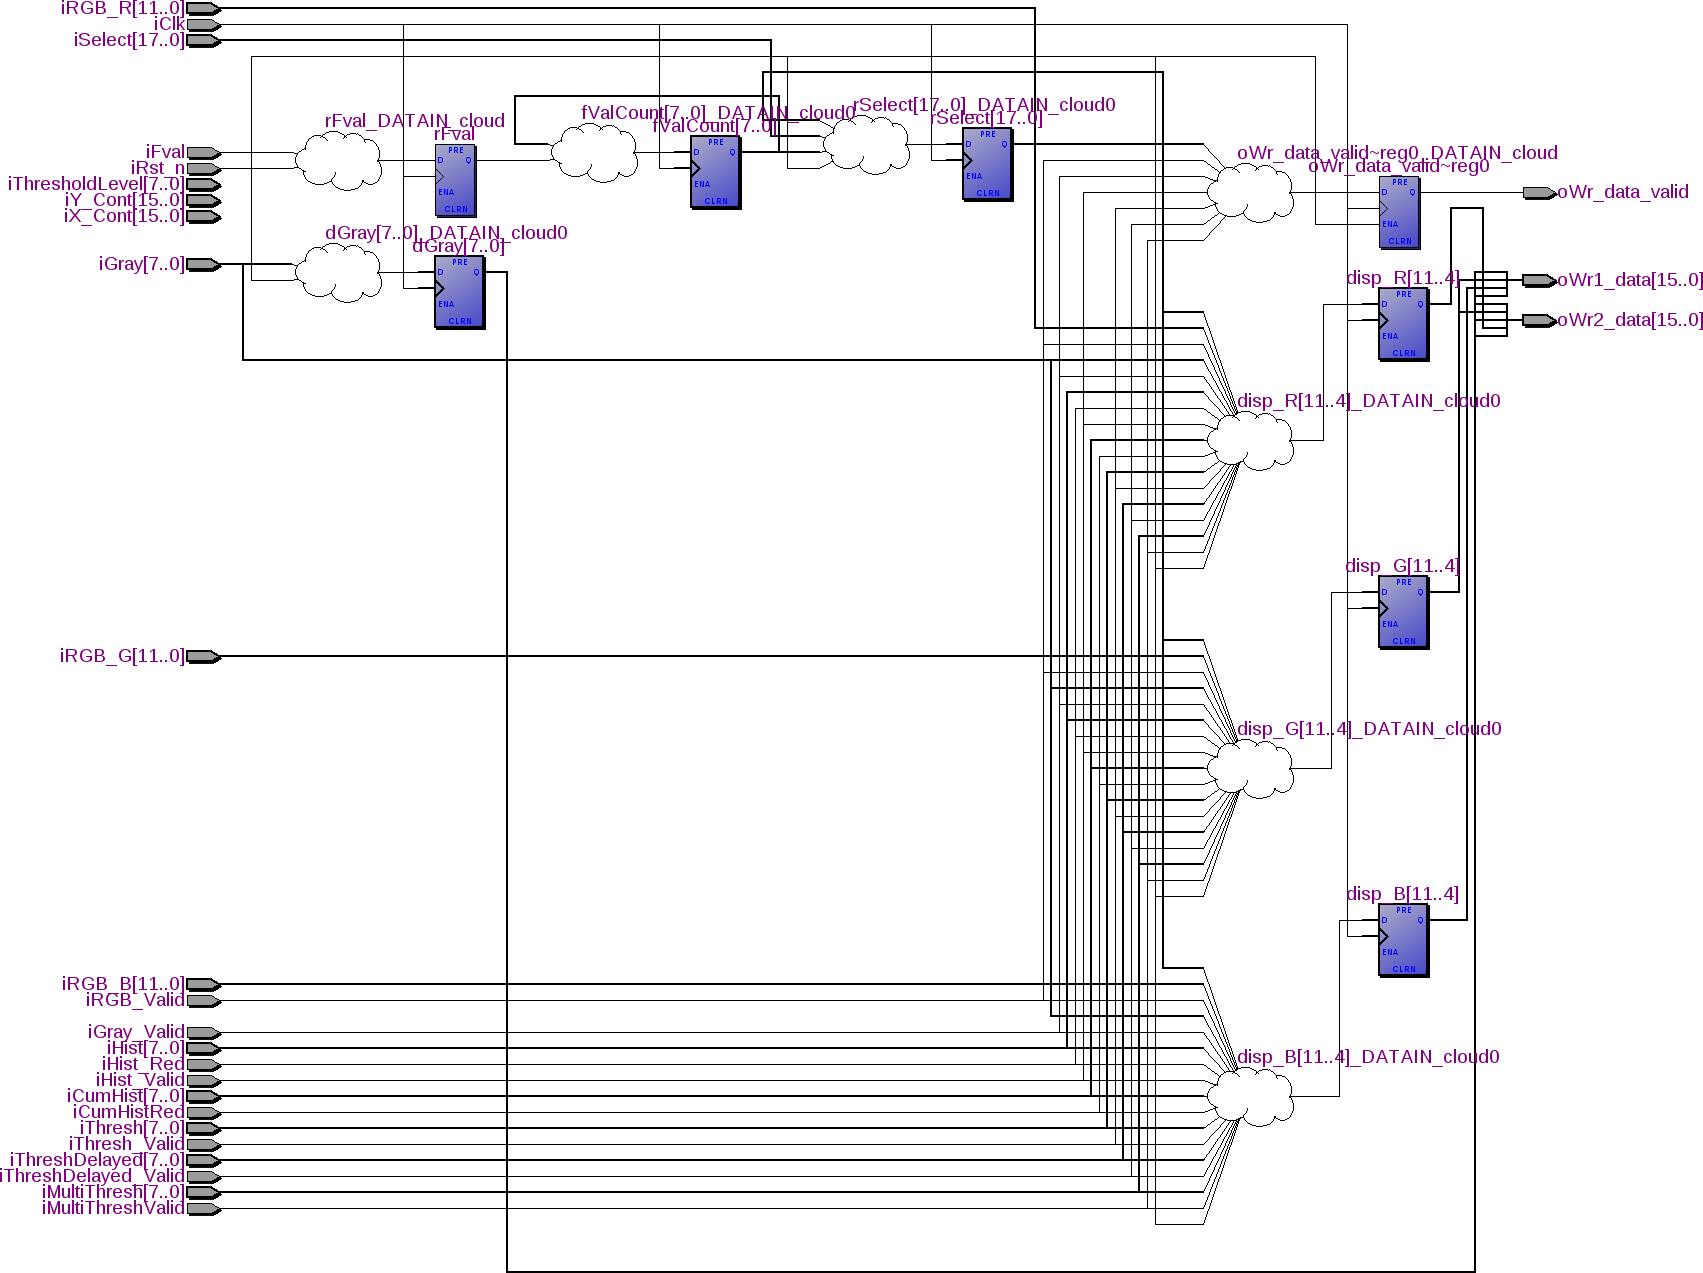
\includegraphics[scale=.8]{Images/ArbitratorRTL.png}}
    \caption{Arbitrator module RTL}
    \label{fig:arbitrator_rtl}
  \end{figure} 
  \subsubsection{RTL Diagram}
    \begin{figure}[H]
    \centering{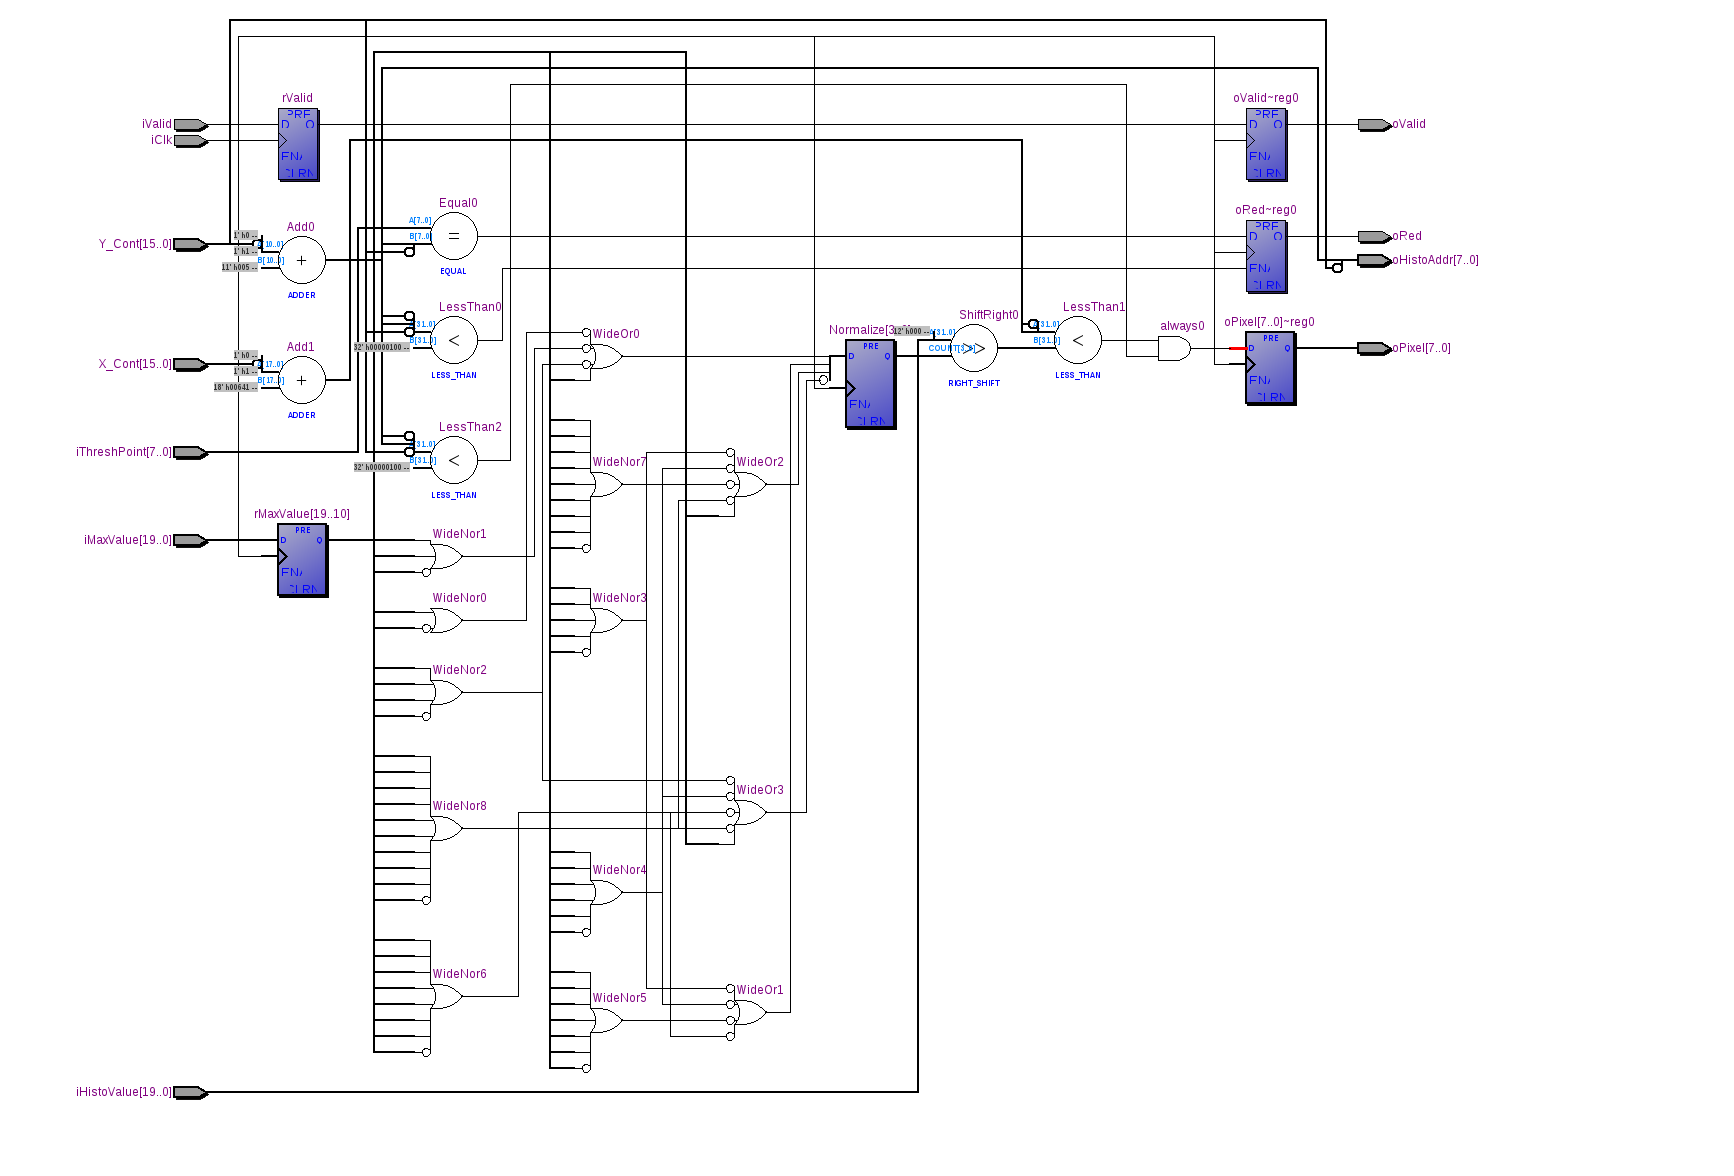
\includegraphics[scale=.8]{Images/HistogramDisplayerRTL.png}}
    \caption{HistogramDisplayer module RTL}
    \label{fig:histogram_displayer_rtl}
  \end{figure}
  
  
  \subsection{High Level Overview}
  \begin{figure}[H]
    \centering{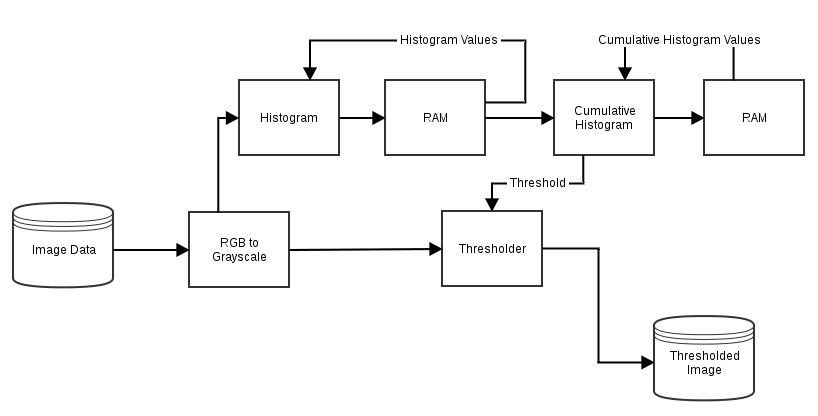
\includegraphics[scale=.65]{Images/HistogramOverview.png}}
    \caption{Overview of the image thresholding process}
    \label{fig:histogram_overview}
  \end{figure}
  
  The toplevel module, \texttt{Total\_Module} is fed RGB values from the camera. Those RGB values are then passed through an RGB to Greyscale conversion to output Greyscale values between 0 and 255. These greyscale values are then passed to the histogram module, which uses an internal RAM to count the number of times each greyscale value is encountered. Once the entire image has been processed, the cumulative histogram module is activated. This module uses its own internal RAM to store the cumulative sum of the histogram. Whilst it calculates the cumulative sum, it checks to see when the cumulative sum passes above the 50th percentile (the point when the sum is less than \(800*480/2\)). It saves this point as the threshold value. On the next frame, this value is then passed through to the thresholder module. The thresholder module uses the threshold it has been given to compare incoming greyscale values. Values that are above the threshold are coloured white, and those below are coloured black.
  
  
  \section{Acknowledgements}
  
  \section{Improvements}
  
  \section{Conclusion}
  
  \newpage
  \newpage
  \section{Appendix C - Testbench Results}
  \subsection{RGB2GRAY}
    In order to test the \texttt{RGB2GRAY} module, the greyscale conversion, a testbench was written that took as inputs the RGB values of an image, and outputted a file containing the grey values calculated by the modelsim simulation. This was then compared to the MATLAB rgb2gray function results. The mean difference between the MATLAB and Verilog functions was only .56, not enough to visibly affect the image output. This was deemed to be well within tolerable bounds.
\begin{figure}[H]
  \centering
  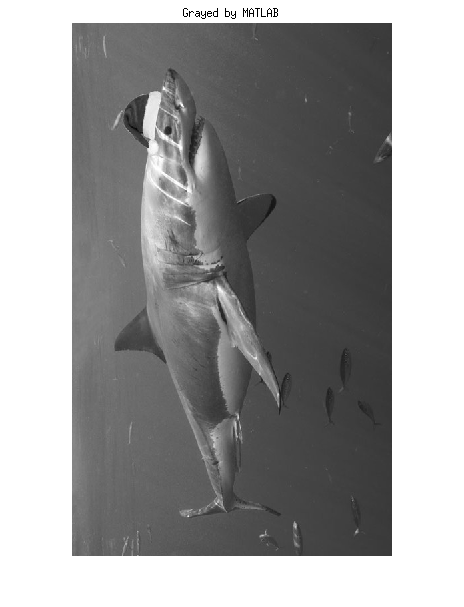
\includegraphics[height=300pt, angle=-90]{Images/RGB2GRAY/MATLAB.png}
  \captionof{figure}{MATLAB rgb2gray result}
\end{figure}
\begin{figure}[H]
  \centering
  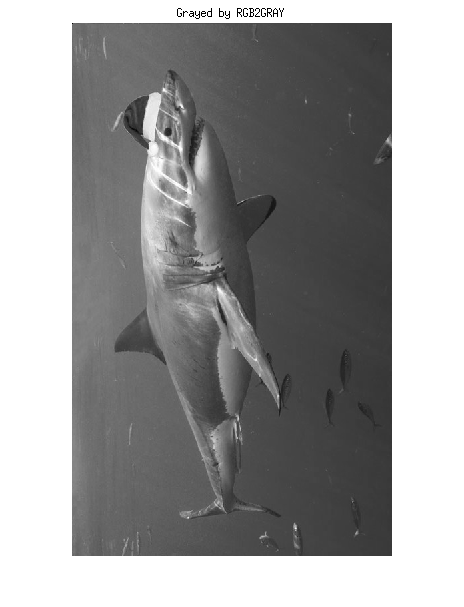
\includegraphics[height=300pt, angle=-90]{Images/RGB2GRAY/Verilog.png}
  \captionof{figure}{RGB2GRAY.v result}
\end{figure}
\begin{figure}[H]
  \centering
  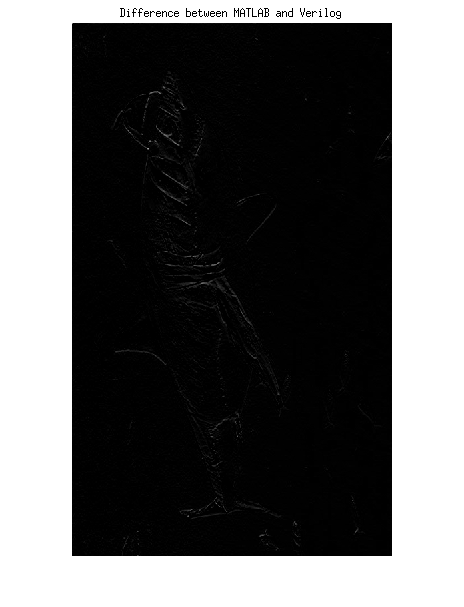
\includegraphics[height=300pt, angle=-90]{Images/RGB2GRAY/Difference.png}
  \captionof{figure}{Difference between the two}
\end{figure}

    
  \newpage
  \subsection{Histogram}
  In order to test the \texttt{Histogram} module, a testbench was written to read in precalculated greyscale values and output a histogram. This histogram was then compared to the histogram generated by matlab. Both histograms are very similar. The mean difference between the two is 3.15.
  \begin{figure}[H]
    \centering{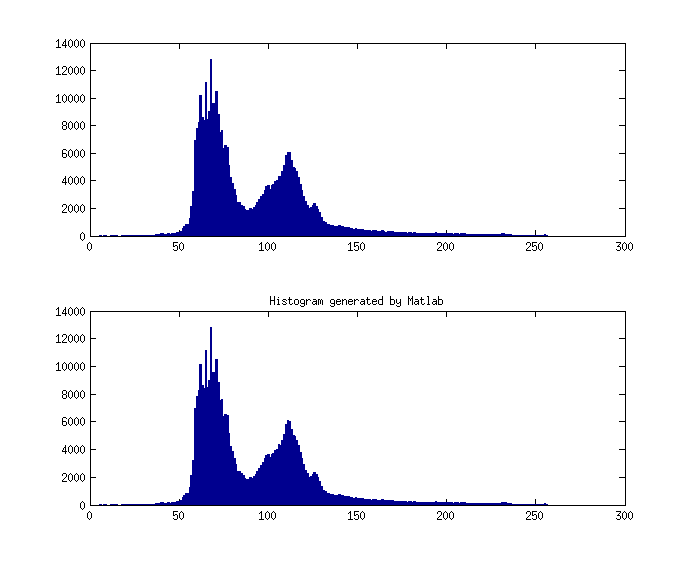
\includegraphics[scale=.8]{Images/HistogramTestbench.png}}
    \caption{Comparison of histogram generated by Histogram module and by matlab}
    \label{fig:histogram_testbench}
  \end{figure} 
  
  \newpage
  \subsection{CumulativeHistogram}d
    In order to test the \texttt{CumulativeHistogram} module, a testbench was written to read in a histogram (generated by \texttt{Histogram} module). The cumulative histogram was then calculated and compared to that generated by matlab. The two cumulative histograms are identical.
  \begin{figure}[H]
    \centering{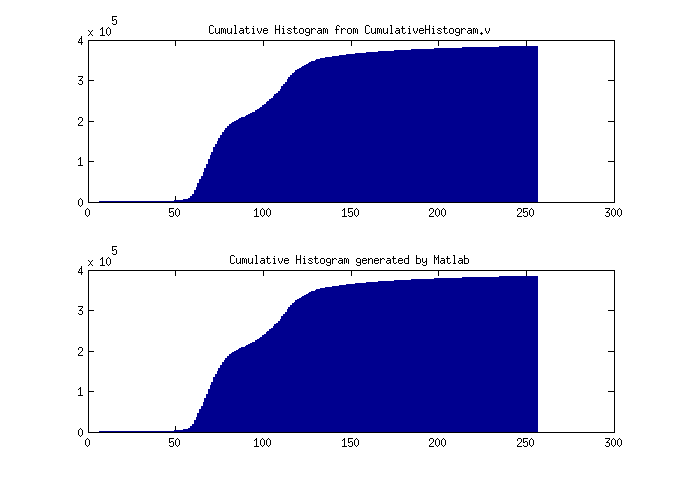
\includegraphics[scale=.8]{Images/CumulativeHistogramTestbench.png}}
    \caption{Comparison of cumulative histogram generated by Cumulative Histogram module and by matlab}
    \label{fig:cumulative_histogram_testbench}
  \end{figure} 
  
  \newpage
  \subsection{Total\_Histogram}
    In order to test the \texttt{Total\_Histogram} module, a testbench was written to read in precalculated greyscale values and output a histogram and a cumulated histogram. The result is the same as those calculated with the separate Histogram and CumulativeHistogram testbenches.
  \begin{figure}[H]
    \centering{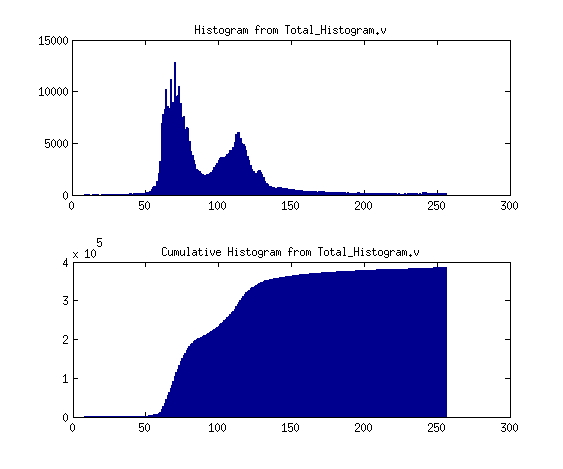
\includegraphics[scale=.8]{Images/Total_HistogramTestbench.png}}
    \caption{Cumulative Histogram and Histogram generated by \texttt{Total\_Histogram} module}
    \label{fig:cumulative_histogram_testbench}
  \end{figure} 
  
  \newpage
  \subsection{HistogramDisplayer}
  In order to test the \texttt{HistogramDisplayer} module, a testbench was written to read in histogram values and output the same image that would be outputted on the LCD screen. MATLAB was then used to display the image.
  \begin{figure}[H]
    \centering{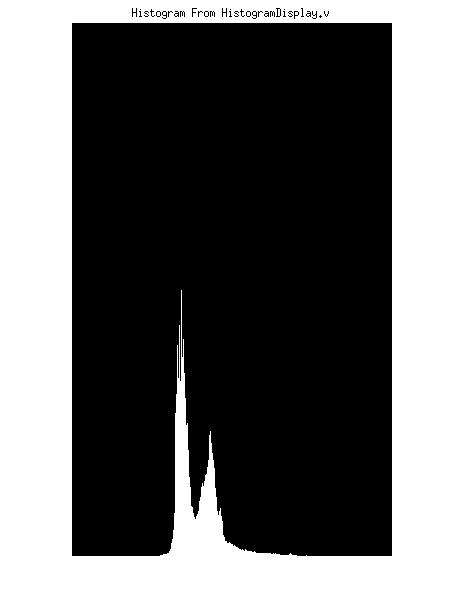
\includegraphics[scale=.8]{Images/HistogramDisplayerTestbench.png}}
    \caption{Image generated by the \texttt{Histogram Displayer module}}
    \label{fig:histogram_displayer_testbench}
  \end{figure} 
  
  \newpage
  \subsection{Total\_Module}
  In order to test \texttt{Total\_Module}, we wrote a testbench that reads in RGB values from a file, then passes those through to an instantiation of \texttt{Total\_Module} along with appropriate data valid signals. The testbench then changes the switch settings and outputs image data to file. A matlab script is used to read in this data and display images. The results are below. Clearly the module behaves correctly for the christmas shark input image, confirming our work in simulation.

\begin{table}[h!]
\begin{center}
\begin{tabular} {c c c}
  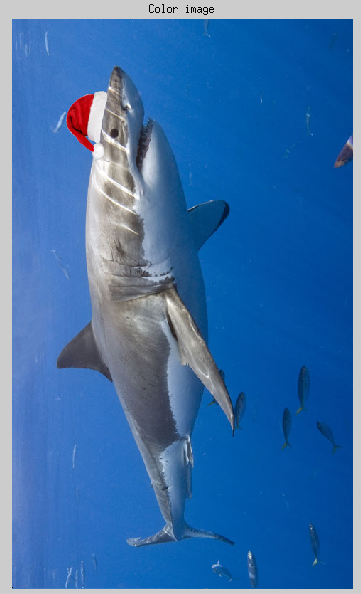
\includegraphics[scale=.52]{Images/TotalModule/RGB.png}
&
  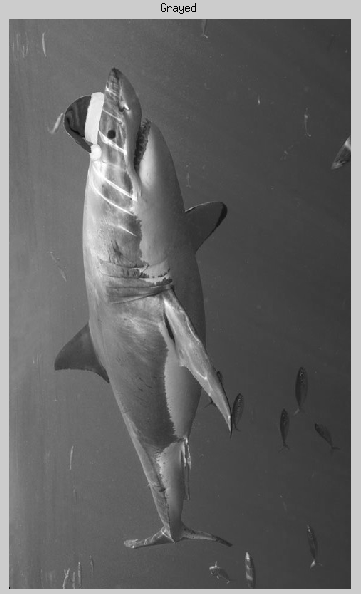
\includegraphics[scale=.52]{Images/TotalModule/Gray.png}
&
  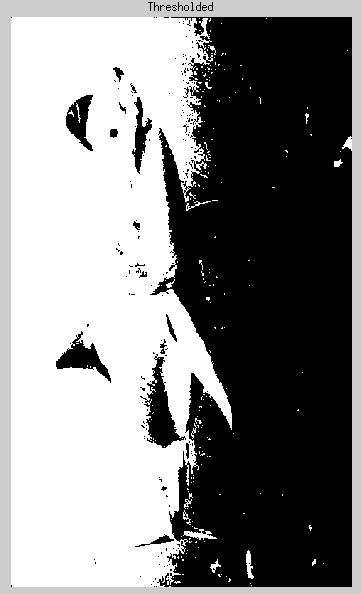
\includegraphics[scale=.52]{Images/TotalModule/Thresholded.png}
\end{tabular}
\end{center}
\captionof{figure}{RGB pass through, grayscale image, and thresholded image}
\end{table}

\begin{table}[h!]
\begin{center}
\begin{tabular} {c c}
  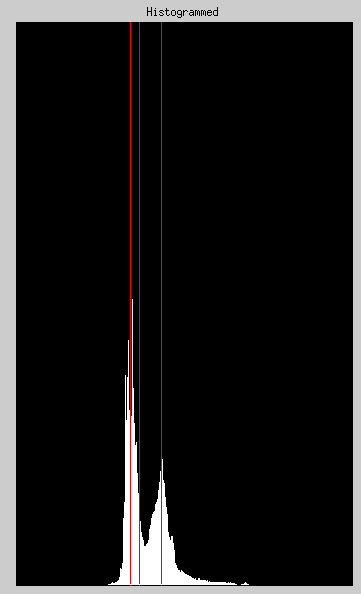
\includegraphics[scale=.8]{Images/TotalModule/Histogrammed.png}
&
  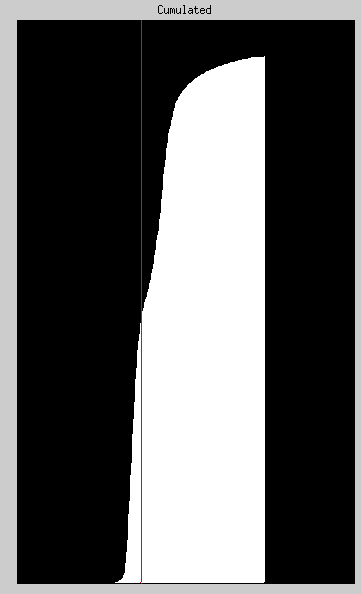
\includegraphics[scale=.8]{Images/TotalModule/Cumulated.png}
\end{tabular}
\end{center}
\captionof{figure}{Histogram and Cumulated Histogram generated by \texttt{Total\_Module}}
\end{table}
  
  \begin{table}[h!]
\begin{center}
\begin{tabular} {c c}
  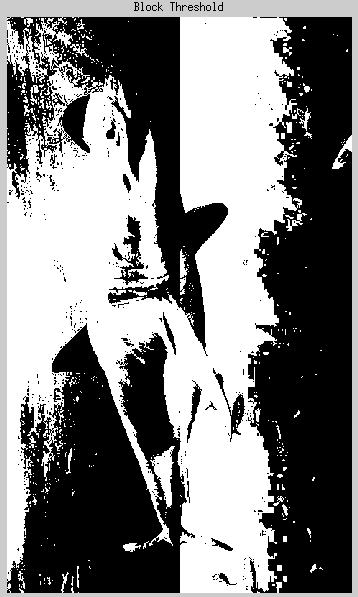
\includegraphics[scale=.8]{Images/TotalModule/BlockThresholded.png}
&
  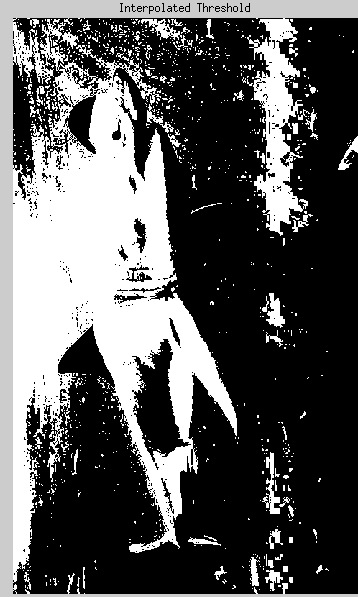
\includegraphics[scale=.8]{Images/TotalModule/SmoothThresholded.png}
\end{tabular}
\end{center}
\captionof{figure}{Histogram and Cumulated Histogram generated by \texttt{Total\_Module}}
\end{table}
  
  
  
  
\end{document}
